\documentclass[12pt]{article}
\usepackage{setspace}       % For setting spacing
\usepackage{titlesec}       % For customizing title styles
\usepackage{tocloft}        % For customizing the table of contents
\usepackage{times}          % Use Times New Roman font
\usepackage[utf8]{inputenc} % Input encoding
\usepackage[margin=1in]{geometry} % Set margins
\usepackage{apacite}        % APA-style references
\usepackage{url}            % For formatting URLs
\usepackage{tikz}
\usetikzlibrary{arrows.meta, shapes.geometric}

% Set 1.5 line spacing
\renewcommand{\baselinestretch}{1.5} 

% Title format
\titleformat{\section}{\normalfont\Large\bfseries}{\thesection}{1em}{}

\begin{document}

% Cover Page
\begin{titlepage}
    \centering
    \vspace*{2in}
    {\Huge \bfseries Predicting the Winner of Chess Games Using Binary Classificaiton Machine Learning Models \\[2in]}
    {\Large Seth Schwiethale \\[0.5in]}
    {\Large December 2, 2024 \\}
    \vfill
\end{titlepage}

% Table of Contents
\newpage
\tableofcontents
\newpage

% Content Sections
\section{Introduction}
Chess has been one of the world's most popular games for centuries. Over 10 years ago, it was estimated that 605 million adults regularly play chess \cite{fidePressRelease2012}. In the intervening years, the popularity of the game has continued to grow alongside the growth of online gaming where Chess.com alone surpassed 20 million members in 2017 \cite{chessMembers}. With so many chess players around the world, when two meet, how might one predict the winner of the game? This paper compares the application of two Machine Learning binary classification algorithms to this question.

Chess competitions and online platforms commonly use the Elo rating system to indicate the relative skill level of players. Elo ratings can be used to predict the outcome of a match \cite{chessElo}. While Elo ratings are calculated based on the outcomes of previous games, the question is whether a learning algorithm can incorporate additional features of a game to improve upon the prediction accuracy of Elo alone.

To perform this analysis, multiple models were trained using two fundamental supervised classification Machine Learning algorithms: Logistic Regression and Decision Trees. The accuracy of these models were then compared to each other and to the accuracy of predictions made based solely on each player's Elo rating.

\section{Research Background}

\subsection{Elo Ratings and Outcome Prediction}
The Elo rating system was created by Arpad Elo and adopted by the U.S. Chess Federation in 1960. ``Each player's Elo rating is represented by a number that reflects that person's results in previous rated games. After each rated game, their ratings are adjusted according to the outcome of the encounter.'' \cite{chessElo}. Given the Elo rating of each player, the expected outcome can be calculated with the following formula:


\[
E_A = \frac{1}{1 + 10^{(R_B - R_A)/400}}
\]

Where $E_A$ is the expectation that player $A$ will win and $R_A$ and $R_B$ are the Elo ratings of players $A$ and $B$, respectively. An $E_A$ value $> 0.5$ predicts that will win with increasing probability up to $E_A == 1$.

\subsection{Binary Classification}

In Machine Learning, classification ``is a problem of automatcially assigning a label to an unlabeled example'' \cite[Chapter 2, Section 2.7]{100MLB}. If the number of possible labels is two ("White wins", "Black wins"), such a classification problem is called binary classification. Though there are three possible outcomes to a chess game: White wins, Black wins or Draw, this study aims specifically to predict a winner, given some set of features describing the characterstics of a specific game, making it a binary classification problem. It is worth noting that, although about 50\% of games end in a draw amongst the highest-rated players \cite{chessBaseDraws}, most of the world's chess players are not professionals and the occurence of draws is much lower, less than 5\% in the data used in this analysis.

\subsection{Logistic Regression}

Logistic Regression is a supervised binary classification learning alogorithm that uses the standard logistic function, often referred to as the sigmoid function $f_{\textbf{w},b}(\textbf{x})$, whose codomain is $(0, 1)$, to represent the probability that an example is labeled 1. Logistic Regression is trained on a dataset using maximum likelihood optimization by a numerical procedure, such as gradient descent \cite[Chapter 9, Section 9.3]{ShalevShwartz2014}.

\[
f_{\textbf{w},b}(\textbf{x}) := \frac{1}{1 + \exp(-(\langle\textbf{w}, \textbf{x}\rangle + b))}
\]

where $z$ is the inner product of two vectors, the example's features $\textbf{x}$ and the model's learned parameters $\textbf{w}$ plus parameter $b$: $z = \langle\textbf{w}, \textbf{x}\rangle + b$. During training, the log-likelihood $LogL_{\textbf{w},b}$ is maximized for the model's parameters:

\[
LogL_{\textbf{w},b} =
\sum_{i=1}^N y_i\ln{f_{\textbf{w},b}(\textbf{x}) + (1-y_i)\ln(1 - f_{\textbf{w},b}(\textbf{x}))}
\]

\noindent Where $y_i$ is the label for example $i$.

\vspace{12pt}After training, the model has parameters $\textbf{w}$ and $b$ that maximize likelihood that the training dataset is according to the resulting model. These parameters are then used to predict labels for a test set. The results are then used to evaluate the accuracy of the model.

\subsubsection{Considerations}Linear Regression is sensitive to the scale of features. Care must be taken when preprocessing the dataset for training to ensure optimal performance.

\subsubsection{Limitations}Linear Regression is best suited for problems where there is a linear relationship between the features and labels. This may prove to be a limitation when considering the kinds of features available to describe a chess game. Some features, such as opening strategy and game duration may not have a linear relation to the outcomes of the game.

\subsection{Decision Trees}

``A decision tree is an acyclic graph that can be used to make decisions'' \cite[Chapter 3, Section 3.3]{100MLB}. Each branch in a decision tree evaluates a feature in the example and branches left if the value is below a threshold and branches right, otherwise. Decisions trees for classification problems can be constsructed by supervised learning. ``The goal is to create a model that predicts the value of a target variable by learning simple decision rules inferred from the data features'' \cite{sklearnDT}. Starting with a root node, the data is split according to each feature and all corresponding thresholds for that feature. The feature and threshold whose resulting split has the largest reduction in entropy (largest information gain) is chosen as the branching feature for that node. The process is repeated recusively to construct the rest of the tree until a stopping condition is met.

Decision tree are easy to visually interpret and, unlike linear regression models, are not sensitive to feature scaling.

\begin{figure}[ht]
\centering
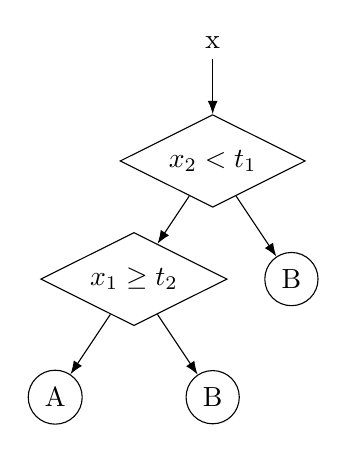
\begin{tikzpicture}[
  edge from parent/.style = {draw, -{Latex}},
  every node/.style = {align=center},
  decision/.style = {draw, diamond, aspect=2, align=center},
  outcome/.style = {draw, circle, align=center},
  level 1/.style = {sibling distance=40mm},
  level 2/.style = {sibling distance=20mm}
]

% Root node
\node {x}
  child {node[decision] {$x_2 < t_1$} % Left child
    child {node[decision] {$x_1 \ge t_2$} % Left child
      child {node[outcome] {A}}
      child {node[outcome] {B}}
    }
    child {node[outcome] {B}}
  };

\end{tikzpicture}
\caption{A simple decision tree demonstrating decision and leaf nodes.}
\label{fig:decision-tree}
\end{figure}

\subsubsection{Considerations}Decision trees can be biased if trained on unbalanced examples. Care must be taken to balance the dateset in preprocessing to reduce bias in the decision tree model.

\subsubsection{Limitation}Decision trees can become complex and are prone to overfitting the training data.

\subsection{Related Work}

Logistic Regression has been used to predict outcomes in many games, such as European-Football \cite{Prasetio2016}, where the authors achieved 69\% accuracy with just a few features and Ice Hockey \cite{Chin2023}, where Logistic Regression outperformed Decision Tree, Support Vector Machine and Artificial Neural Network models used as benchmarks from prior work.

\section{Research and Methods}
This is where the setup content goes.

\section{Materials and Data Sources}
This is where Materials and Data Sources goes.

\section{Results}
This is where the results go.

\section{Discussion and Conclusions}
This is where the conclusion goes.

% References in APA format
\newpage
\bibliographystyle{apacite}
\bibliography{references}  % Ensure there is a file named references.bib with your bibliography entries.

\end{document}